%% LaTeX-Beamer template for KIT design
%% by Erik Burger, Christian Hammer
%% title picture by Klaus Krogmann
%%
%% version 2.1
%%
%% mostly compatible to KIT corporate design v2.0
%% http://intranet.kit.edu/gestaltungsrichtlinien.php
%%
%% Problems, bugs and comments to
%% burger@kit.edu

\documentclass[18pt]{beamer}

%% SLIDE FORMAT

% use 'beamerthemekit' for standard 4:3 ratio
% for widescreen slides (16:9), use 'beamerthemekitwide'
% for widescreen slide without sidebar use 'beamerthemekitwidenosidebar'

\usepackage{templates/beamerthemekit}
\usepackage{graphicx}
%\usepackage{templates/beamerthemekitwide}
%\usepackage{templates/beamerthemekitwidenosidebar}

% use this to disable the latex beamer navigation symbols
%\beamertemplatenavigationsymbolsempty


%% TITLE PICTURE

% if a custom picture is to be used on the title page, copy it into the 'logos'
% directory, in the line below, replace 'mypicture' with the 
% filename (without extension) and uncomment the following line
% (picture proportions: 63 : 20 for standard, 169 : 40 for wide
% *.eps format if you use latex+dvips+ps2pdf, 
% *.jpg/*.png/*.pdf if you use pdflatex)

%\titleimage{mypicture}

%% TITLE LOGO

% for a custom logo on the front page, copy your file into the 'logos'
% directory, insert the filename in the line below and uncomment it

\titlelogo{logo_teco}

% (*.eps format if you use latex+dvips+ps2pdf,
% *.jpg/*.png/*.pdf if you use pdflatex)

%% TikZ INTEGRATION

% use these packages for PCM symbols and UML classes
% \usepackage{templates/tikzkit}
% \usepackage{templates/tikzuml}

% the presentation starts here

\title[Proposal Bachelorarbeit]{Proposal: Klassifikation von respiratorischen Ereignissen mit Earables und maschinellem Lernen}
\subtitle{Professor: Michael Beigl, Betreuer: Tobias Röddiger}
\author{David Laubenstein}

\institute{Lehrstuhl Pervasive Computing Systems}

% Bibliography

\usepackage[citestyle=authoryear,bibstyle=numeric,hyperref,backend=biber]{biblatex}
\addbibresource{templates/example.bib}
\bibhang1em

\begin{document}
\selectlanguage{ngerman}

%title page
\begin{frame}
\titlepage
\end{frame}

% --------------------------- 1. Folie PIBA ----------------------------------

\section{PIBA}
\subsection{Problem}
\begin{frame}{Problem}
%insert picture from sleepApneaDeclaration
    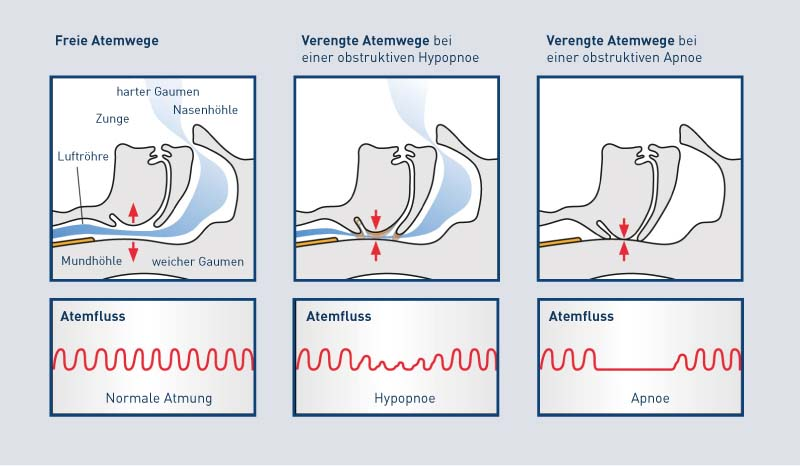
\includegraphics[scale=0.4]{logos/was-passiert-bei-schlafapnoe}
\end{frame}

\begin{frame}{Problem}
%insert picture from sleeping labor
    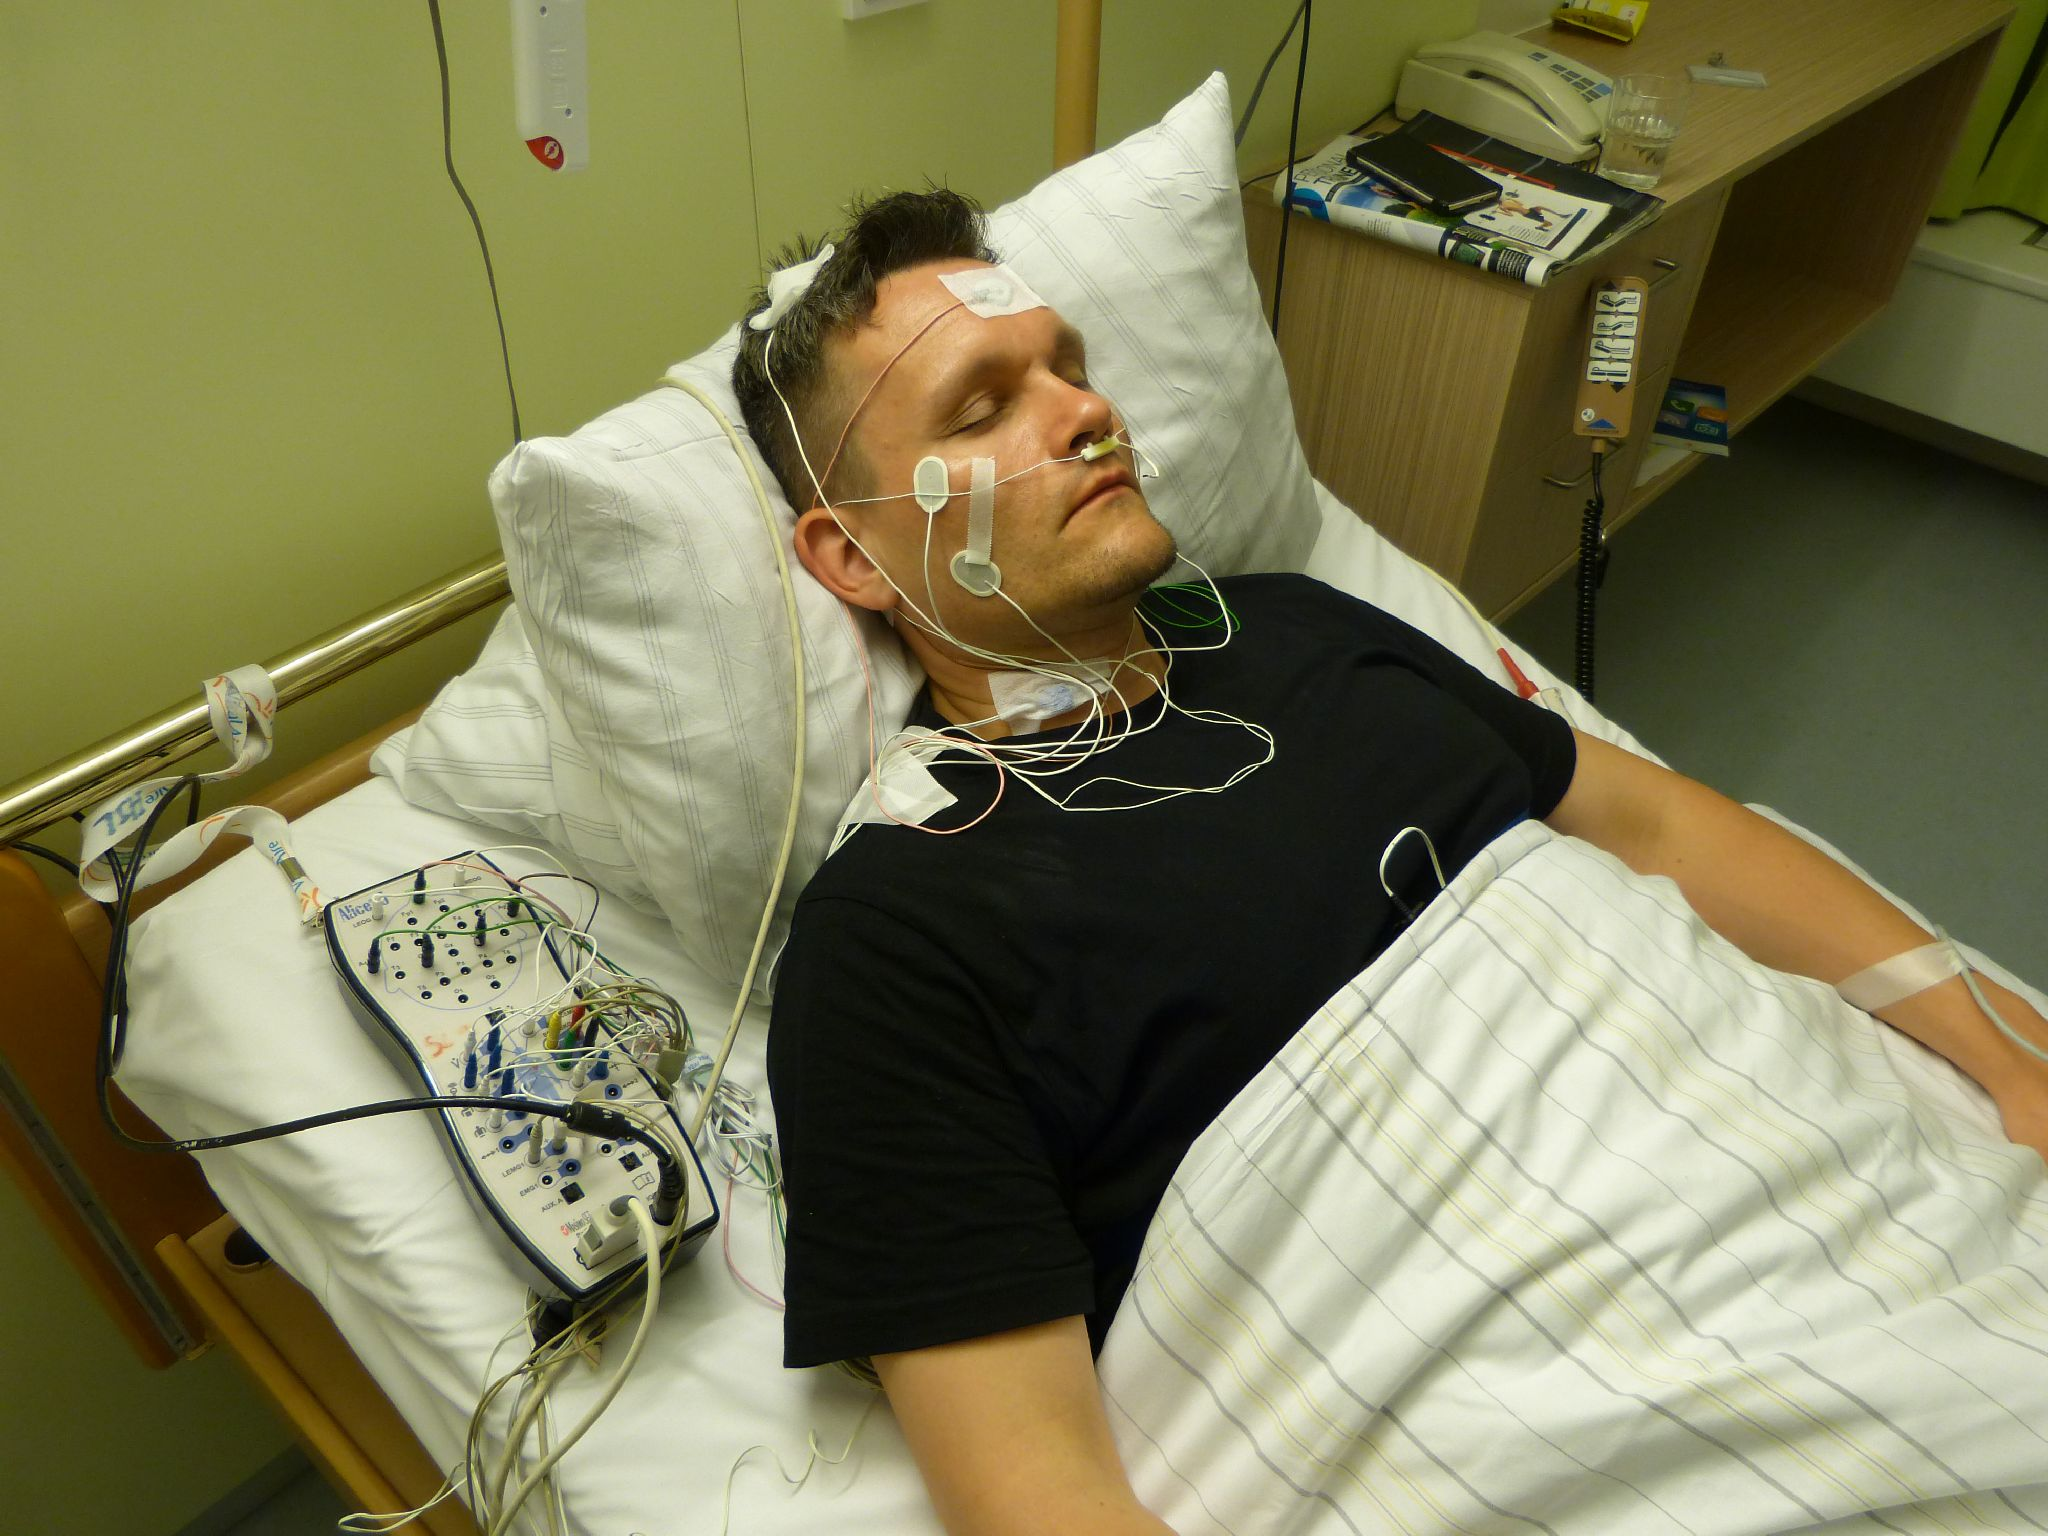
\includegraphics[scale=0.12]{logos/sleepLabor}
\end{frame}

\subsection{Idee}
\begin{frame}{Idee}
%insert picture from Earbuds for solution to diagnose this 
    \begin{columns}[T] % align columns
	\begin{column}{.48\textwidth}
	    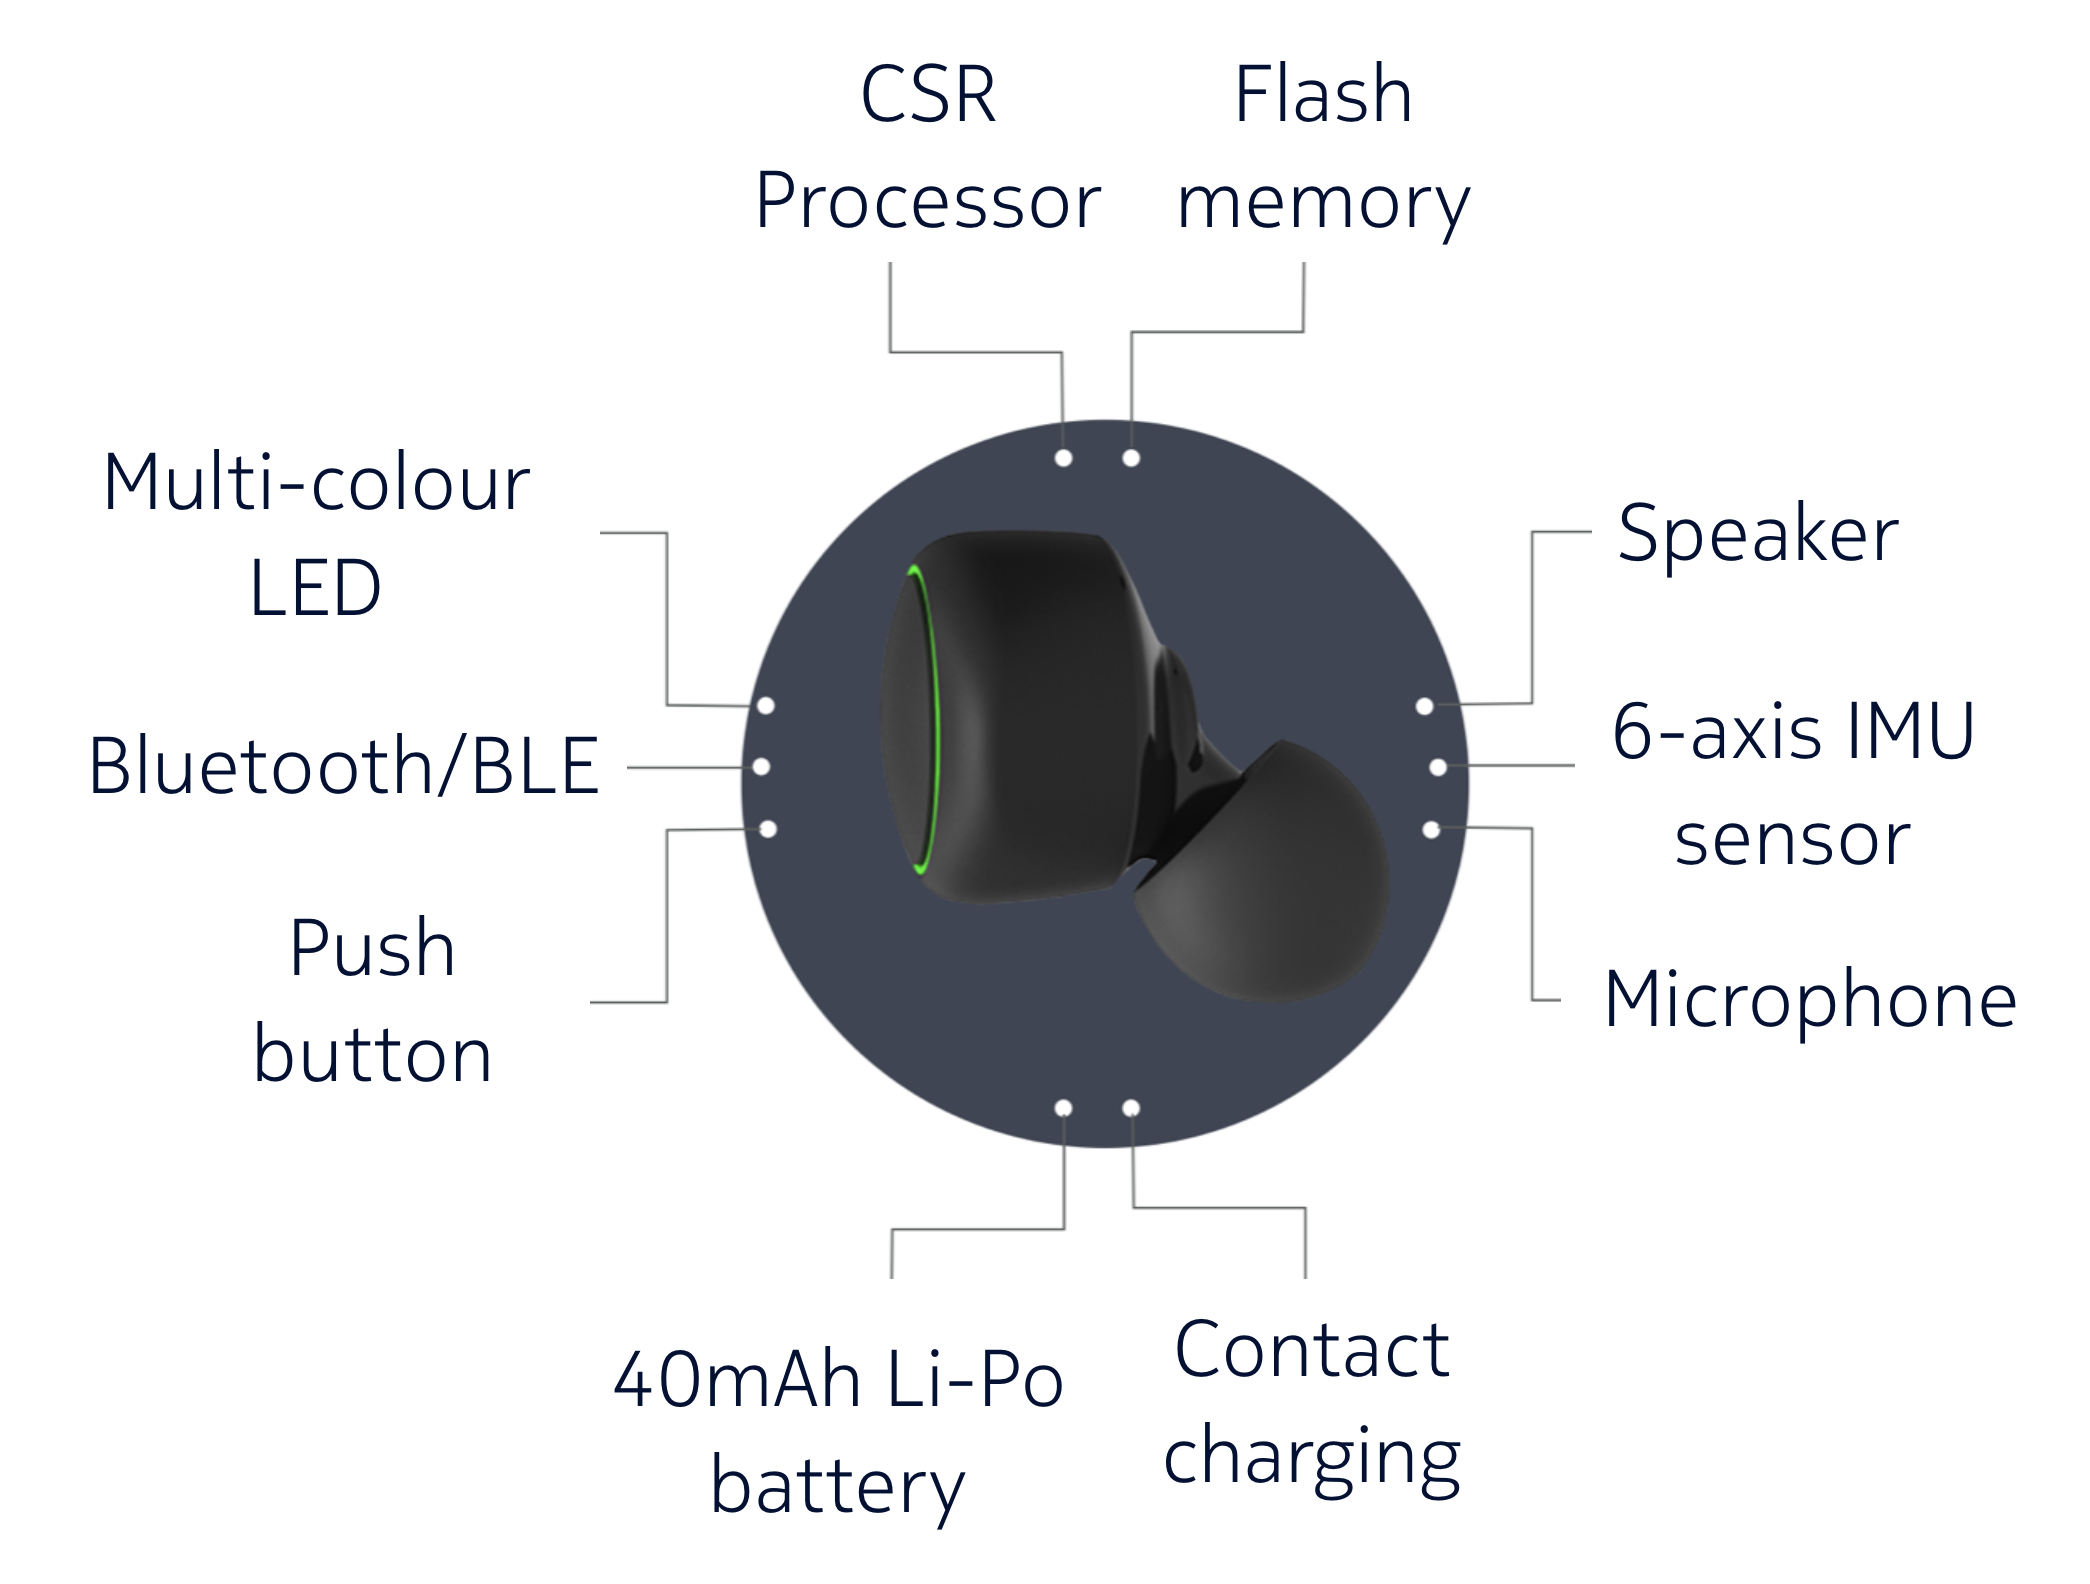
\includegraphics[scale=0.15]{logos/esense}
	\end{column}%
	\hfill%
	\begin{column}{.48\textwidth}
	    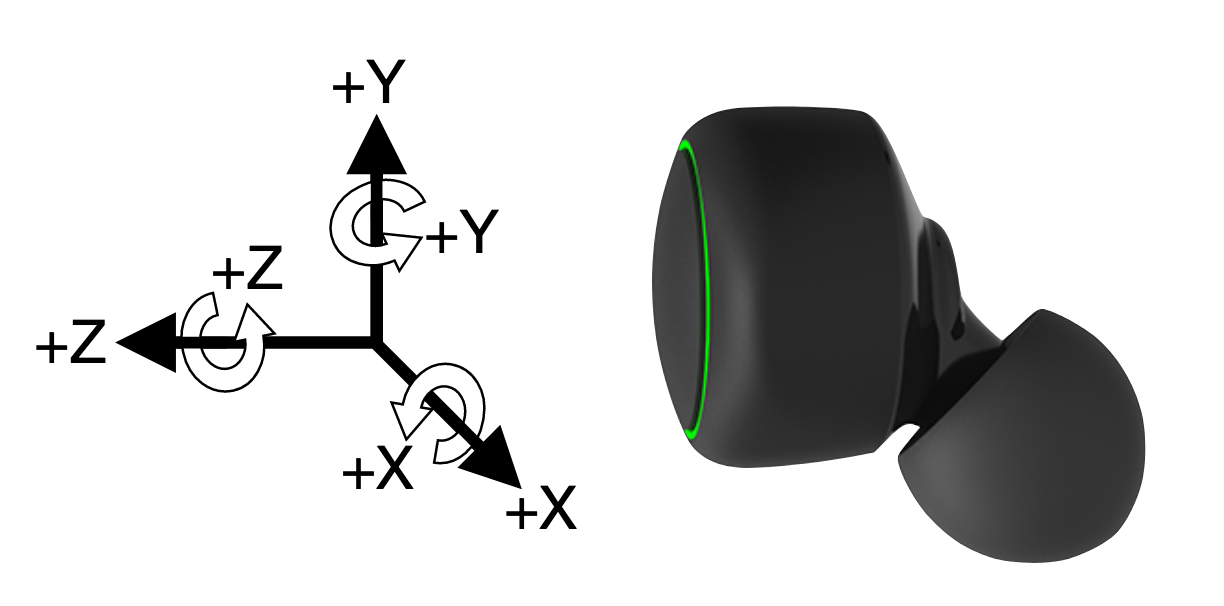
\includegraphics[scale=0.25]{logos/esense2}
	\end{column}%
	\end{columns}
	Vorteil:
	\begin{itemize}
		\item Test kann unkompliziert zuhause durchgeführt werden
		\item Sensoren bereits heute in Kopfhörern vorhanden (Apple AirPods)
	\end{itemize}
\end{frame}

\subsection{Action}
\begin{frame}{Action}
Phasen der Bachelorarbeit
    \begin{columns}[T] % align columns
	\begin{column}{.48\textwidth}
	    \begin{itemize}
	    	\item Nutzerstudie, Datensatz
	    	\item Evaluation von maschinellen Lernverfahren
	    	\item Schreibphase
	    \end{itemize}
	\end{column}%
	\hfill%
	\begin{column}{.48\textwidth}
		\includegraphics<1>[width=1.0\textwidth]{logos/esense2}
		\includegraphics<2>[height=1.2\textwidth]{logos/smartphone}
		\includegraphics<3>[width=1.0\textwidth]{logos/machineLearning}
		\includegraphics<4>[width=1.0\textwidth]{logos/writeBA}
	\end{column}%
    \end{columns}
\end{frame}

% ----------------------- 2. Folie Umsetzung ihres Lösungsansatzes -------------
\section{Fragestellungen}
\begin{frame}{Fragestellungen}
Fragestellungen zur Nutzerstudie
\begin{itemize}
	\item Welche Informationen über die Probanden sollen gesammelt werden
	\begin{itemize}
		\item Art des Earable-Aufsatzes
		\item allg. Information über Proband
		\begin{itemize}
			\item Geschlecht, Gewicht, all. Fitness, Schlafrythmus, ... 
		\end{itemize}
		\item Interview nach Nutzerstudie
		\begin{itemize}
			\item Tragekomfort der Earables?
			\item Wohlbefinden währrend der Studie
		\end{itemize}
	\end{itemize}
\end{itemize}
Evaluation von maschinellen Lernverfahren zur Klassifikation
\begin{itemize}
	\item Welche maschinellen Lernverfahren gibt es?
\end{itemize}
\end{frame}


% ----------------------- 3. Folie Geplante Evaluation -------------
\section{Geplante Evaluation}
\begin{frame}{Geplante Evaluation}
\begin{itemize}
	\item Vergleich verschiedener maschineller Lernverfahren
	\item Vergleich mit aktuellem Industriestandard (Schlaflabor)
\end{itemize}
\end{frame}

% ----------------------- 4. Folie Zusammenfassung -------------
\section{Zusammenfassung}
\begin{frame}{Zusammenfassung}
	\begin{itemize}
		\item Problem: Diagnose von Schlafstörungen
		\begin{itemize}
			\item Earables als Schlaflaborersatz
		\end{itemize}
		\item Nutzerstudie, Datensatz
		\item Maschinelle Lernverfahren zur Klassifikation
		\item Evaluation
	\end{itemize}
\end{frame}

% ----------------------- 5. Folie Zusatz Nutzerstudie -------------
\begin{frame}{Nutzerstudie: Definitionen}
	\begin{itemize}
		\item Positionen
		\begin{itemize}
			\item liegend auf dem Rücken
			\item liegend auf dem Bauch
			\item seitlich liegend
		\end{itemize}
		\item Simulation Schlafstörung
		\begin{itemize}
			\item Proband hält Luft an
			\item simuliert zentrales Apnoe
		\end{itemize}
	\end{itemize}
	\end{frame}
	
\begin{frame}{Nutzerstudie: Ablauf}
Pro Liegeposition wird folgender Ablauf durchgeführt:
\begin{itemize}
	\item 60 Sekunden atmen
	\item 10 Sekunden luft anhalten
	\item 60 Sekunden atmen
	\item 20 Sekunden luft anhalten
	\item 60 Sekunden atmen
	\item 30 Sekunden luft anhalten
	\item 120 Sekunden atmen
\end{itemize}
\end{frame}


\appendix
\beginbackup

\begin{frame}[allowframebreaks]{References}
\begin{itemize}
	\item https://www.deutsche-familienversicherung.de/ratgeber/artikel/das-schlafapnoe-syndrom/
	\item https://www.extratipp.com/bilder/2017/06/16/8406482/1320911264-schlaflabor-hofheim-krankenhaus-schlafen-traeumen-atemaussetzer-selbsttest-testbericht.jpg
\end{itemize}
\printbibliography
\end{frame}

\backupend

\end{document}
